\documentclass[]{article}
\usepackage[utf8]{inputenc}
\usepackage[portuguese]{babel}
\usepackage{graphicx}
\title{O método de Euler e a solução exata}
\author{Helena Isola Guimarães}
\begin{document}
\maketitle
Em um problema de valor inicial, temos como objetivo encontrar a solução da equação diferencial y que 
satisfaça as condições iniciais dadas por $y(x_0)=y_0$ e $y’(x0)=y1$, onde o $y’(x_0)$ pode ser obtido a 
partir do valor $y_0$, e assim podemos ir sucessivamente até encontrarmos o valor desejado de $y_0$. 

Podemos utilizar o método de euler para resolver equações diferenciais como os exemplos abaixo:

\subparagraph*{Exemplo 1}
\begin{equation}
    y' = x + y  (1)  e  y(0) = 1
\end{equation}
Onde, de maneira analítica resolvemos utilizando o método do fator integrante:

\[\mu (x).y' = \mu (x).x + \mu (x).y\]
\[\mu (x).y' - \mu (x).y = \mu (x).x \]
\[(\mu (x).y)' = \mu (x).x\]
\[\mu '(x) =(-1). \mu (x)\]
\[\mu '(x)\mu (x) = -1\]
\[\mu '(x)\mu (x)dx = -1 dx\]
\[\ln (x) = -x +c_0\]
\[(x) = e^{-x+c_0}\]

Voltando agora na equação inicial que possui forma e sendo $c_0 = 0$:

\[(\mu (x).y)' = \mu (x).x\]
\[ e-x.y  = e-x.x dx \]
\[e-x.y  = -x.e-x - e-x+c\]
\[y = -x -1 + ce-\]

Sabendo que $y(0) = 1$, podemos encontrar o valor de c substituindo na equação (2) os valores iniciais:
\[1 = - 0 -1 + \frac{c}{e^0}\] 		
ou seja,  \[c = 2\]

Portanto a solução será:
\[y = -x -1 + 2 \]
\[y = 1 - x  \]

Assim, temos que (2.1) será a solução exata de (1). Utilizando um código com o método de Euler, obtemos o seguinte resultado de comparação ao plotar as duas saídas quando temos n = 10 (intervalos entre os valores de x).

\begin{figure}
    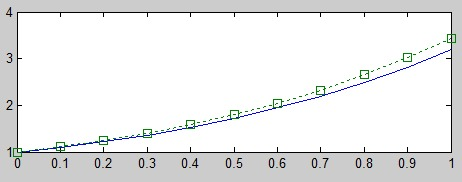
\includegraphics[width=\linewidth]{euler1.jpeg}
    \caption{y'=x+y}
    \label{fig:euler1}
\end{figure}

\end{document}